
% Copyright (C) 2014-2017 by Thomas Auzinger <thomas@auzinger.name>

% added by rfischer: oneside, to avoid ugly intendation
\documentclass[draft,final,oneside]{vutinfth} % Remove option 'final' to obtain debug information.

% Load packages to allow in- and output of non-ASCII characters.
\usepackage{lmodern}        % Use an extension of the original Computer Modern font to minimize the use of bitmapped letters.
\usepackage[T1]{fontenc}    % Determines font encoding of the output. Font packages have to be included before this line.
\usepackage[utf8]{inputenc} % Determines encoding of the input. All input files have to use UTF8 encoding.

% Extended LaTeX functionality is enables by including packages with \usepackage{...}.
\usepackage{amsmath}    % Extended typesetting of mathematical expression.
\usepackage{amssymb}    % Provides a multitude of mathematical symbols.
\usepackage{mathtools}  % Further extensions of mathematical typesetting.
\usepackage{microtype}  % Small-scale typographic enhancements.
\usepackage[inline]{enumitem} % User control over the layout of lists (itemize, enumerate, description).
\usepackage{multirow}   % Allows table elements to span several rows.
\usepackage{booktabs}   % Improves the typesettings of tables.
\usepackage{subcaption} % Allows the use of subfigures and enables their referencing.
\usepackage[ruled,linesnumbered,algochapter]{algorithm2e} % Enables the writing of pseudo code.
\usepackage[usenames,dvipsnames,table]{xcolor} % Allows the definition and use of colors. This package has to be included before tikz.
\usepackage{nag}       % Issues warnings when best practices in writing LaTeX documents are violated.
\usepackage{todonotes} % Provides tooltip-like todo notes.
\usepackage{hyperref}  % Enables cross linking in the electronic document version. This package has to be included second to last.
\usepackage[acronym,toc]{glossaries} % Enables the generation of glossaries and lists fo acronyms. This package has to be included last.
\usepackage[usenames,dvipsnames]{pstricks}
\usepackage{epsfig}
\usepackage{pst-grad} % For gradients
\usepackage{pst-plot} % For axes
\usepackage[space]{grffile} % For spaces in paths
\usepackage{etoolbox} % For spaces in paths
\makeatletter % For spaces in paths
\patchcmd\Gread@eps{\@inputcheck#1 }{\@inputcheck"#1"\relax}{}{}
\makeatother
% Define convenience functions to use the author name and the thesis title in the PDF document properties.
\newcommand{\authorname}{Robert Fischer} % The author name without titles.
\newcommand{\thesistitle}{Deep Learning of Humor from Gary Larson's Cartoons} % The title of the thesis. The English version should be used, if it exists.

% Set PDF document properties
\hypersetup{
    pdfpagelayout   = TwoPageRight,           % How the document is shown in PDF viewers (optional).
    linkbordercolor = {Melon},                % The color of the borders of boxes around crosslinks (optional).
    pdfauthor       = {\authorname},          % The author's name in the document properties (optional).
    pdftitle        = {\thesistitle},         % The document's title in the document properties (optional).
    pdfsubject      = {Deep Learning},              % The document's subject in the document properties (optional).
    pdfkeywords     = {a, list, of, keywords} % The document's keywords in the document properties (optional).
}

\setpnumwidth{2.5em}        % Avoid overfull hboxes in the table of contents (see memoir manual).
\setsecnumdepth{subsection} % Enumerate subsections.

\nonzeroparskip             % Create space between paragraphs (optional).
\setlength{\parindent}{0pt} % Remove paragraph identation (optional).

\makeindex      % Use an optional index.
\makeglossaries % Use an optional glossary.
%\glstocfalse   % Remove the glossaries from the table of contents.

% Set persons with 4 arguments:
%  {title before name}{name}{title after name}{gender}
%  where both titles are optional (i.e. can be given as empty brackets {}).
\setauthor{}{\authorname}{BSc.}{male}
\setadvisor{Dr.}{Horst Eidenberger}{Assoc. Prof.}{male}

% For bachelor and master theses:
%\setfirstassistant{Pretitle}{Forename Surname}{Posttitle}{male}
%\setsecondassistant{Pretitle}{Forename Surname}{Posttitle}{male}
%\setthirdassistant{Pretitle}{Forename Surname}{Posttitle}{male}

% For dissertations:
%\setfirstreviewer{Pretitle}{Forename Surname}{Posttitle}{male}
%\setsecondreviewer{Pretitle}{Forename Surname}{Posttitle}{male}

% For dissertations at the PhD School and optionally for dissertations:
%\setsecondadvisor{Pretitle}{Forename Surname}{Posttitle}{male} % Comment to remove.

% Required data.
\setaddress{Stauraczgasse 8/13 \\ 1050 Wien \\ Österreich}
\setregnumber{01425684}
\setdate{14}{05}{2018} % Set date with 3 arguments: {day}{month}{year}.
\settitle{\thesistitle}{Deep Learning of Humor from Gary Larson's Cartoons} % Sets English and German version of the title (both can be English or German). If your title contains commas, enclose it with additional curvy brackets (i.e., {{your title}}) or define it as a macro as done with \thesistitle.
\setsubtitle{}{} % Sets English and German version of the subtitle (both can be English or German).

% Select the thesis type: bachelor / master / doctor / phd-school.
% Bachelor:
%\setthesis{bachelor}
%
% Master:
\setthesis{master}
\setmasterdegree{dipl.} % dipl. / rer.nat. / rer.soc.oec. / master
%
% Doctor:
%\setthesis{doctor}
%\setdoctordegree{rer.soc.oec.}% rer.nat. / techn. / rer.soc.oec.
%
% Doctor at the PhD School
%\setthesis{phd-school} % Deactivate non-English title pages (see below)

% For bachelor and master:
\setcurriculum{Artificial Intelligence and Game Engineering}{Artificial Intelligence and Game Engineering} % Sets the English and German name of the curriculum.

% For dissertations at the PhD School:
\setfirstreviewerdata{Affiliation, Country}
\setsecondreviewerdata{Affiliation, Country}


\begin{document}

\frontmatter % Switches to roman numbering.
% The structure of the thesis has to conform to
%  http://www.informatik.tuwien.ac.at/dekanat

\addtitlepage{naustrian} % German title page (not for dissertations at the PhD School).
\addtitlepage{english} % English title page.
\addstatementpage

%\begin{danksagung*}
%\todo{Ihr Text hier.}
%\end{danksagung*}

%\begin{acknowledgements*}
%\todo{Enter your text here.}
%\end{acknowledgements*}

%\begin{kurzfassung}
%\todo{Ihr Text hier.}
%\end{kurzfassung}

%\begin{abstract}
%\todo{Enter your text here.}
%\end{abstract}

% Select the language of the thesis, e.g., english or naustrian.
\selectlanguage{english}

% Add a table of contents (toc).
\tableofcontents % Starred version, i.e., \tableofcontents*, removes the self-entry.

% Switch to arabic numbering and start the enumeration of chapters in the table of content.
\mainmatter

\chapter{Problem Definition}

\begin{figure}[ht]
	\centering
  	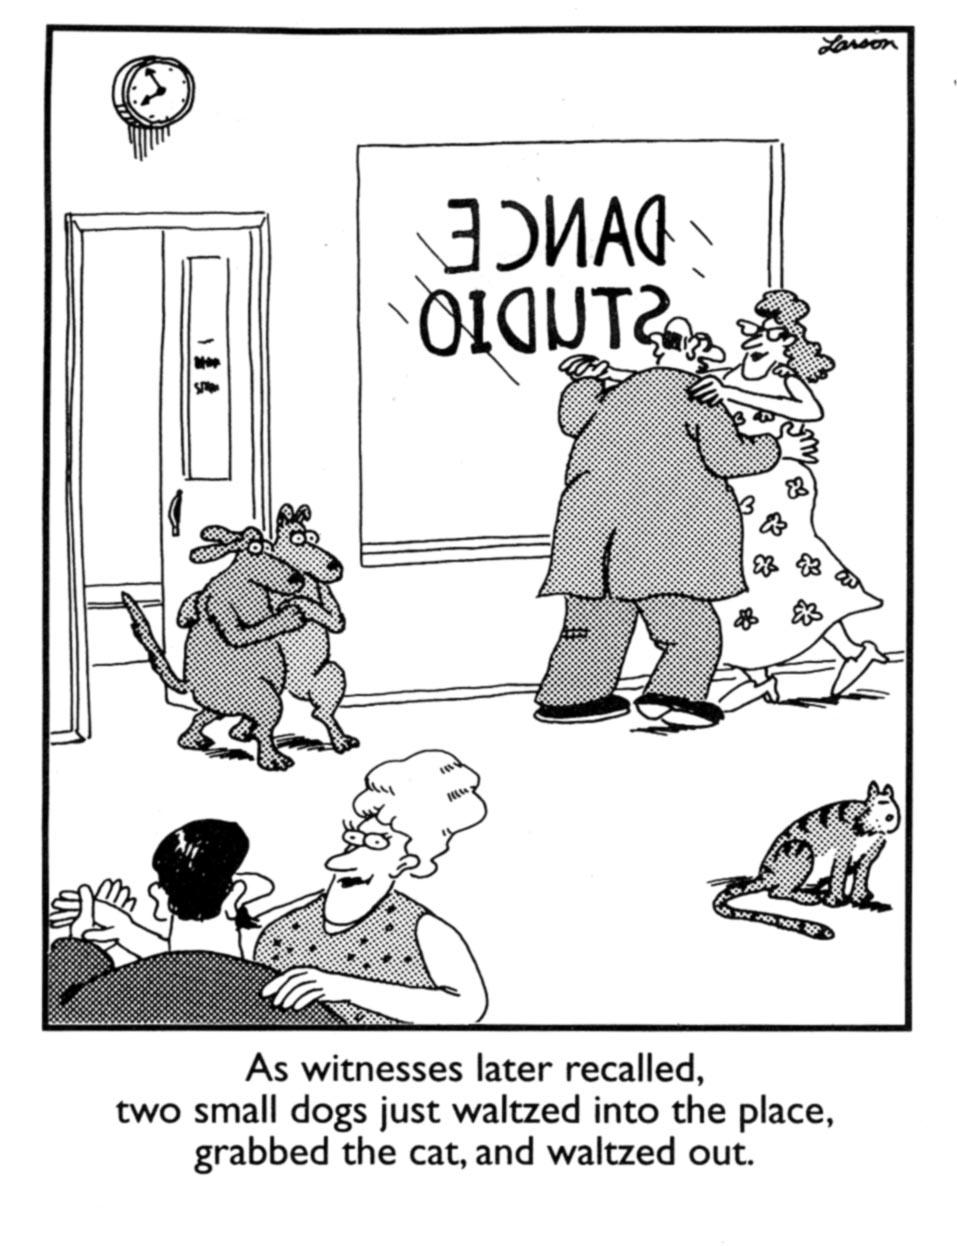
\includegraphics[width=0.5\textwidth,natwidth=957,natheight=1246]{./graphics/example_cartoon.png}
	\caption{Cartoon by Gary Larson}
	\label{fig1}
\end{figure}

The main goal of this diploma thesis is to research whether computers are capable of understanding human humor by learning Gary Larson's cartoons. This is done by applying several Deep Learning techniques. \\


Previous approaches of computational humor mainly focused on written text \cite{Yang2015HumorRA}\cite{Bamman2015ContextualizedSD}\cite{HumoristBot}, research of humor using deep learning is still in its infancy. With the advent of deep learning and convolutional neural networks (=CNN) in recent years \cite{Druzhkov2016}, images may now be taken into consideration as well and similarly recurrent neural networks have been improving the state-of-the-art in several natural language processing disciplines \cite{reviewRNN}. \\

\textbf {Cartoon Classification:} \quad Convolutional neural networks are mostly applied to real world pictures, because most problems of computer vision are in this domain. The question remains whether they are also capable of analyzing cartoons and if there are ways on how to improve CNNs for this type of images. An experiment of regular image classification will be adapted for Gary Larson's cartoons. The traditional image classification task using the CIFAR-10 data set, where categorizing images into ten classes (cat, dog, airplane, etc.) will be adapted for his cartoons. Classification should range from animal cartoons, culture dish cartoons to harder categories, such as cartoons that contain a depiction of god. The original task is already solved with convolutional neural networks \cite{dogsvscats}, the question remains if the same is true for Gary Larson's cartoons. \\

\textbf {Humor Classification:} \quad Often cartoons by Gary Larson also contain a punchline, which will be extracted using existing optical image recognition solutions. The extracted text has to be considered when trying to understand humor. Here recurrent neural networks, especially Long Short-Term Memory networks, will be applied (TODO: REF). The main problem of these networks, is that they have the tendency to overfit to the training data \cite[page 4]{reviewRNN}, which is a major challenge to be overcome. \\

Another goal is to evaluate the resulting neural networks. Hidden inside them, there might be some interesting insights about human humor, especially since deep neural networks are inspired by the human brain and function similarly \cite{Cichy2016}. Maybe some neural network layers will have their own dedicated function, or there will be a cow-detection neuron inside the network? These and related questions will be investigated in the present thesis.

\chapter{Expected Results}

The main outcome of this thesis is a machine learning pipeline which is able to classify a cartoon by funniness. This pipeline consists of a pre-processing phase, training phase and testing phase. A similar pipeline for the cartoon classification task will also be developed, but it will be adapted to multilabel classification. Classes include different types of animals (cats, dogs, horses, etc.), different settings (culture dish, stone age, outer space, etc.) and more semantically challenging classes (contains god appearance, contains marriage conflict, etc.). \\

Secondly, the model will be evaluated rigorously and the hope is to find some new insights into the neural structure of human humor. For example, if this thesis shows the existence of a neuron which fires if and only if a cow is visible, this could imply, that the human brain also has neurons that function similarly \cite{Cichy2016}. The existence of layers that serve certain functions might also be worth investigating. \\

If the network performs well in the test phase, then this is a very strong indicator, that the deep neural networks are actually able to learn the human humor. This would open many new research possibilities. \\

Another important result is an annotated ground truth, which will be facilitated to train the classifiers. This ground truth may be used for future research as well, such as comparing humor between Gary Larson and other authors.

\chapter{Methodology and Approach}
\section {Literature Research}
First the available literature will be researched. The goal is to have a broad understanding and knowledge of state-of-the-art in machine learning, deep neural network architectures, human humor and human perception. \\

\section {Pre-Processing}
In this step the ground truth will be created: A data set of several thousand cartoons exists, but these cartoons need to be pre-processed in such a way that a neural network can be trained on this data set: The punchlines have to be extracted, the pictures need to be normalized and bad examples filtered. Additionally manual labelling of cartoons is necessary: For the humor classification the funniness of a cartoon has to be annotated with a numerical value and for the cartoon classification task a binary n-tuple that describes which type of cartoon is illustrated. \\

\section {Humor Classification}
Given this data set, based on previous classifications, the goal is to predict how funny a previously unseen cartoon is. This is done by training multiple machine learning classifiers. Important to note is the fact, that humor is subjective, so the generated model might only be applicable for individuals. \\

For the visual component of a cartoon, a convolutional neural network will be trained, as they have been applied very successfully in various image classification tasks \cite{dogsvscats}. If and how deep neural networks have to be adapted to work with cartoons will be researched during the thesis. Possibly a generative adversarial approach may be implemented. \cite{gan}  \\

A punchline analysis will be implemented using recurrent neural networks and other natural language processing techniques. Prime candidate are Long Short-Term Memory networks. Here several different variations exist with widely different combinations of activation functions and layers (TODO REF). The goal is to find the best performing network for the given task. Other techniques will be considered as well, such as Gated Recurrent Units (TODO REF).

Finally both neural networks are merged together using another, possibly more traditional, machine learning classifier. \\

\section {Cartoon Classification}

Similar to the humor classification approach, a deep neural network that classifies cartoons by different categories will be trained. The question remains how to handle cartoons properly using deep neural networks, additionally data augmenting techniques might be implemented to avoid overfitting. \\

Gary Larson has many reoccurring themes, such as different settings (culture dish, stone age, outer space, etc.), reoccurring animals (dogs, cats, horses, etc.) or other phenomena (god appearing, marriage conflict, etc.). This makes training a deep neural network which is able to classify these categories an interesting task. On the quest to the best classifier, first different convolutional neural networks will be applied, possibly a generative adversarial approach may also be implemented. (TODO REF)

\section {Evaluation}

During the evaluation, the trained models are applied to the test set (a set of previously unknown data). The humor classification task has one out of many choices per cartoon, hence it is considered a multiclass classification task, on the other hand the cartoon classification task has many out of many choices per cartoon (since a cartoon can contain for example a cat and a dog), hence it is considered a multilabel multiclass classification task. \\

Evaluation will be mostly based on a confusion matrix in order to calculate an average F-score \cite{Powers2008EvaluationFP}. If the classes are not evenly distributed special considerations are necessary. Additionally ROC curves may be also used for evaluation \cite{Hand2001}. 

\chapter{State of the Art}

At the time of writing this proposal there has been little research in the area of computational humor using deep learning. Deep Learning of Audio and Language Features for Humor Prediction \cite{Bertero2016DeepLO} is the only notable paper in this area, which uses deep learning for punchline detection based on dialogue and audio of a US sitcom. This approach ignores the visual component entirely and also does not use Long Short-Term Memory networks. \\

For image classification various types of convolutional neural networks are state-of-the-art \cite{dogsvscats}. Recurrent Long Short-Term Memory networks are being used very successfully for various natural language processing tasks as well \cite{reviewRNN}. \\

Previous approaches of computational humor include sarcasm \cite{Bamman2015ContextualizedSD}, joke detection \cite{Yang2015HumorRA} or rule-based humor \cite{HumoristBot}. All of these attempts treated humor as isolated chunks of text, while also ignoring the visual component entirely.

\section{Neural Networks}

\begin{figure}[ht]
	\centering
	\scalebox{.5}{
	\begin{pspicture}(0,-4.227907)(12.08,4.227907)
\definecolor{colour0}{rgb}{0.70980394,0.70980394,0.70980394}
\definecolor{colour1}{rgb}{0.8627451,0.5686275,0.2784314}
\definecolor{colour2}{rgb}{0.5137255,0.78039217,0.5411765}
\rput[bl](0.0,-4.227907){Input Layer}
\rput[bl](10.0,-4.227907){Output Layer}
\rput[bl](5.2,-4.227907){Hidden Layers}
\psline[linecolor=black, linewidth=0.04](1.5906976,2.6837208)(2.8930233,3.427907)
\psline[linecolor=black, linewidth=0.04](1.5906976,2.6837208)(2.8930233,1.5674418)
\psline[linecolor=black, linewidth=0.04](1.5906976,2.6837208)(2.8930233,-0.29302326)
\psline[linecolor=black, linewidth=0.04](1.5906976,2.6837208)(2.8930233,-2.339535)
\psline[linecolor=black, linewidth=0.04](1.5906976,0.82325584)(2.8930233,3.427907)
\psline[linecolor=black, linewidth=0.04](1.5906976,0.82325584)(2.8930233,1.5674418)
\psline[linecolor=black, linewidth=0.04](1.5906976,0.82325584)(2.8930233,-0.29302326)
\psline[linecolor=black, linewidth=0.04](1.5906976,0.82325584)(2.8930233,-2.339535)
\psline[linecolor=black, linewidth=0.04](1.5906976,-1.2232558)(2.8930233,3.427907)
\psline[linecolor=black, linewidth=0.04](1.5906976,-1.2232558)(2.8930233,1.5674418)
\psline[linecolor=black, linewidth=0.04](1.5906976,-1.2232558)(2.8930233,-0.29302326)
\psline[linecolor=black, linewidth=0.04](1.5906976,-1.2232558)(2.8930233,-2.339535)
\psline[linecolor=black, linewidth=0.04](4.009302,3.6139536)(5.311628,3.6139536)
\psline[linecolor=black, linewidth=0.04](4.009302,3.6139536)(5.311628,1.5674418)
\psline[linecolor=black, linewidth=0.04](4.009302,3.6139536)(5.311628,-0.47906977)
\psline[linecolor=black, linewidth=0.04](4.009302,3.6139536)(5.311628,-2.339535)
\psline[linecolor=black, linewidth=0.04](4.009302,1.5674418)(5.311628,3.6139536)
\psline[linecolor=black, linewidth=0.04](4.009302,1.5674418)(5.311628,1.5674418)
\psline[linecolor=black, linewidth=0.04](4.009302,1.5674418)(5.311628,-0.47906977)
\psline[linecolor=black, linewidth=0.04](4.009302,1.5674418)(5.311628,-2.339535)
\psline[linecolor=black, linewidth=0.04](4.009302,-0.47906977)(5.311628,3.6139536)
\psline[linecolor=black, linewidth=0.04](4.009302,-0.47906977)(5.311628,1.5674418)
\psline[linecolor=black, linewidth=0.04](4.009302,-0.47906977)(5.311628,-0.47906977)
\psline[linecolor=black, linewidth=0.04](4.009302,-0.47906977)(5.311628,-2.339535)
\psline[linecolor=black, linewidth=0.04](4.009302,-2.339535)(5.311628,3.6139536)
\psline[linecolor=black, linewidth=0.04](4.009302,-2.339535)(5.311628,1.5674418)
\psline[linecolor=black, linewidth=0.04](4.009302,-2.339535)(5.311628,-0.47906977)
\psline[linecolor=black, linewidth=0.04](4.009302,-2.339535)(5.311628,-2.339535)
\psline[linecolor=black, linewidth=0.04](6.427907,3.6139536)(7.7302327,3.6139536)
\psline[linecolor=black, linewidth=0.04](6.427907,3.6139536)(7.7302327,1.5674418)
\psline[linecolor=black, linewidth=0.04](6.427907,3.6139536)(7.7302327,-0.47906977)
\psline[linecolor=black, linewidth=0.04](6.427907,3.6139536)(7.7302327,-2.339535)
\psline[linecolor=black, linewidth=0.04](6.427907,1.5674418)(7.7302327,3.6139536)
\psline[linecolor=black, linewidth=0.04](6.427907,1.5674418)(7.7302327,1.5674418)
\psline[linecolor=black, linewidth=0.04](6.427907,1.5674418)(7.7302327,-0.47906977)
\psline[linecolor=black, linewidth=0.04](6.427907,1.5674418)(7.7302327,-2.5255814)
\psline[linecolor=black, linewidth=0.04](6.427907,-0.47906977)(7.7302327,3.6139536)
\psline[linecolor=black, linewidth=0.04](6.427907,-0.47906977)(7.7302327,1.5674418)
\psline[linecolor=black, linewidth=0.04](6.427907,-0.47906977)(7.7302327,-0.47906977)
\psline[linecolor=black, linewidth=0.04](6.427907,-0.47906977)(7.7302327,-2.5255814)
\psline[linecolor=black, linewidth=0.04](6.427907,-2.339535)(7.7302327,3.6139536)
\psline[linecolor=black, linewidth=0.04](6.427907,-2.339535)(7.7302327,1.5674418)
\psline[linecolor=black, linewidth=0.04](6.427907,-2.339535)(7.7302327,-0.47906977)
\psline[linecolor=black, linewidth=0.04](6.427907,-2.339535)(7.7302327,-2.339535)
\psellipse[linecolor=black, linewidth=0.04, fillstyle=solid,fillcolor=colour0, dimen=outer](5.9255815,1.5767442)(0.6511628,0.6511628)
\psline[linecolor=black, linewidth=0.04](8.846512,3.6139536)(10.148837,2.8697674)
\psline[linecolor=black, linewidth=0.04](8.846512,3.6139536)(10.148837,0.82325584)
\psline[linecolor=black, linewidth=0.04](8.846512,3.6139536)(10.148837,-1.2232558)
\psline[linecolor=black, linewidth=0.04](8.846512,1.5674418)(10.148837,2.8697674)
\psline[linecolor=black, linewidth=0.04](8.846512,1.5674418)(10.148837,0.82325584)
\psline[linecolor=black, linewidth=0.04](8.846512,1.5674418)(10.148837,-1.2232558)
\psline[linecolor=black, linewidth=0.04](8.846512,-0.47906977)(10.148837,0.82325584)
\psline[linecolor=black, linewidth=0.04](8.846512,-0.47906977)(10.148837,-1.2232558)
\psline[linecolor=black, linewidth=0.04](8.846512,-0.47906977)(10.148837,2.8697674)
\psline[linecolor=black, linewidth=0.04](8.846512,-2.339535)(10.148837,2.8697674)
\psline[linecolor=black, linewidth=0.04](8.846512,-2.339535)(10.148837,0.82325584)
\psline[linecolor=black, linewidth=0.04](8.846512,-2.339535)(10.148837,-1.2232558)
\psellipse[linecolor=black, linewidth=0.04, fillstyle=solid,fillcolor=colour1, dimen=outer](10.725581,2.7767441)(0.6511628,0.6511628)
\psellipse[linecolor=black, linewidth=0.04, fillstyle=solid,fillcolor=colour1, dimen=outer](10.725581,0.7767441)(0.6511628,0.6511628)
\psellipse[linecolor=black, linewidth=0.04, fillstyle=solid,fillcolor=colour1, dimen=outer](10.725581,-1.2232559)(0.6511628,0.6511628)
\psellipse[linecolor=black, linewidth=0.04, fillstyle=solid,fillcolor=colour0, dimen=outer](8.325582,-2.4232557)(0.6511628,0.6511628)
\psellipse[linecolor=black, linewidth=0.04, fillstyle=solid,fillcolor=colour0, dimen=outer](8.325582,3.576744)(0.6511628,0.6511628)
\psellipse[linecolor=black, linewidth=0.04, fillstyle=solid,fillcolor=colour0, dimen=outer](8.325582,1.5767442)(0.6511628,0.6511628)
\psellipse[linecolor=black, linewidth=0.04, fillstyle=solid,fillcolor=colour0, dimen=outer](8.325582,-0.4232558)(0.6511628,0.6511628)
\psellipse[linecolor=black, linewidth=0.04, fillstyle=solid,fillcolor=colour0, dimen=outer](5.9255815,3.576744)(0.6511628,0.6511628)
\psellipse[linecolor=black, linewidth=0.04, fillstyle=solid,fillcolor=colour0, dimen=outer](5.9255815,-0.4232558)(0.6511628,0.6511628)
\psellipse[linecolor=black, linewidth=0.04, fillstyle=solid,fillcolor=colour0, dimen=outer](5.9255815,-2.4232557)(0.6511628,0.6511628)
\psellipse[linecolor=black, linewidth=0.04, fillstyle=solid,fillcolor=colour2, dimen=outer](1.1255814,0.7767441)(0.6511628,0.6511628)
\psellipse[linecolor=black, linewidth=0.04, fillstyle=solid,fillcolor=colour2, dimen=outer](1.1255814,-1.2232559)(0.6511628,0.6511628)
\psellipse[linecolor=black, linewidth=0.04, fillstyle=solid,fillcolor=colour2, dimen=outer](1.1255814,2.7767441)(0.6511628,0.6511628)
\psellipse[linecolor=black, linewidth=0.04, fillstyle=solid,fillcolor=colour0, dimen=outer](3.5255814,3.576744)(0.6511628,0.6511628)
\psellipse[linecolor=black, linewidth=0.04, fillstyle=solid,fillcolor=colour0, dimen=outer](3.5255814,1.5767442)(0.6511628,0.6511628)
\psellipse[linecolor=black, linewidth=0.04, fillstyle=solid,fillcolor=colour0, dimen=outer](3.5255814,-0.4232558)(0.6511628,0.6511628)
\psellipse[linecolor=black, linewidth=0.04, fillstyle=solid,fillcolor=colour0, dimen=outer](3.5255814,-2.4232557)(0.6511628,0.6511628)
\end{pspicture}
}
	\caption{Fully Connected Feed Forward Neural Network}
	\label{fig:feedforward}
\end{figure}

Part of the reason why neural networks are so powerful, especially deep neural networks, stems from their flexibility. They can adapt to lots of different domains very easily. Illustrated at figure \ref{fig:feedforward} is a simple fully connected feedforward neural network. A neural network generally consists of multiple neurons, layers and connections. \\

The following neural network introduction is cited from Pattern Recognition and Machine Learning by Christopher M. Bishop \cite{bishop}. \\ 

A neural network can be seen as a series of functional transformations. Given the input $x_1, ..., x_D$ and $M$ connections the input layer can be described as:
\begin{equation}
a_j = \sum_{i=1}^{D} w_{ji}^{(1)} + w_{j0}^{(1)}
\end{equation}

where $j = 1, ..., M$. $w_{ji}^{(n)}$ is usually referred to as weights and $w_{j0}^{(n)}$ as biases. $a_j$ is called an activation, which is then transformed using a nonlinear, differentiable activation function $h(\cdot)$:
\begin{equation}
z_j = h(a_j)
\end{equation}
where depending on the problem different activation functions are applied, for example $h(x) = tanh(x)$ or $h(x) = \sigma(x)$ where
\begin{equation}
\sigma(x) = \dfrac {1} {1 + e^{-x}}
\end{equation}
for the first hidden layer the following values are linearly combined:
\begin{equation}
a_k = \sum_{i=1}^{M} w_{kj}^{(2)} + w_{k0}^{(2)}
\end{equation}

where $k = 1, ..., K$ is the total number of outputs of the first hidden layer. The same procedure is repeated for all hidden layers. The final result for the output layer is usually obtained by applying a softmax activation function. \\

The neural network is then trained by applying a gradient descent optimization. For more information regarding this algorithm Machine Learning by Christopher M. Bishop \cite{bishop} is recommended. 

\subsection{Convolutional Neural Networks}
The following is summarizing several papers (TODO).

Based on feedforward neural networks convolutional neural networks emerged. A convolutional neural network is a deep neural network, since it consists of multiple hidden layers, which are configured differently compared to traditional neural networks. Additionally to fully connected hidden layers pooling and convolutional layers are added. \\

Convolutional layers apply a convolution on each pixel. A convolution is a weighted sum between two functions. The first function is the input signal and the second function a filter kernel. Instead of each neuron being connected to all other neurons, they are connected to a relatively small local subset of the neurons in the previous layer, which allows them to recognize certain local patterns (e.g.: edges). Also in contrast to fully connected layers: The kernel is shared among the neurons (Parameter Sharing), since the recognized features should not depend on their position in the input image. \\

Pooling layers are applied after convolutional layers. Their goal is to reduce the complexity of CNNs. Pooling neurons are connected to a local subset of the neurons in the previous layer, but without weights, biases or a kernel. The input is transformed by a function. A typical pooling layer is Max Pooling, where the result is the maximum value of all incoming connections. \\

Fully connected layers are usually the last layers of a CNN, their task is to perform classification based on the extracted features of the previous layers. \\

\subsection{Recurrent Neural Networks}
Recurrent Neural Networks (RNN) allow neural networks to be applied on sequences, by allowing cycles in the topology of the network. Usually a RNN consists of multiple units, such as Long Short-Term Memory networks (LSTM), Gates recurrent unit, etc. The focus of this thesis will primarily be on LSTM networks. \\

Each architecture has different benefits and applicable domains. Even among LSTM networks there is lots of variation. In fact recurrent neural networks are so powerful they are even turing complete \cite{seigelmann:computation}. The success of today's speech recognition is driven by RNN networks \cite{googlespeech}. One of the reasons why LSTMs are so powerful compared to other architectures is due to their design, which avoids the vanishing gradient problem \cite {vanishinggradient}.\\

The most simple LSTM unit consists of a memory cell with input and output gates. Inside the LSTM a self-recurrent connection exist but are kept in check by the gates. For a more detailed architecture overview Long Short-Term Memory by Hochreiter Schmidhuber is recommended \cite{hochreiter}.



\chapter{Relation to Master Study}
The master study Artificial Intelligence and Game Engineering has several courses that cover the topic of machine- and deep learning:

\begin{itemize}
\item 183.663, VU, Deep  Learning  for  Visual  Computing
\item 184.702, VU, Machine Learning
\item 188.501, VU, Similarity Modeling 1
\item 188.498, VU, Similarity Modeling 2
\item 188.980, VU, Advanced Information Retrieval
\item 186.143, UE, Informationsvisualisierung 
\item 186.141, VO, Informationsvisualisierung 
\end{itemize}

%\chapter{Introduction}
%\todo{Enter your text here.}

%\chapter{Additional Chapter}
%\todo{Enter your text here.}

\backmatter

% Use an optional list of figures.
% \listoffigures % Starred version, i.e., \listoffigures*, removes the toc entry.

% Use an optional list of tables.
% \cleardoublepage % Start list of tables on the next empty right hand page.
% \listoftables % Starred version, i.e., \listoftables*, removes the toc entry.

% Use an optional list of alogrithms.
% \listofalgorithms
% \addcontentsline{toc}{chapter}{List of Algorithms}

% Add an index.
% \printindex

% Add a glossary.
% \printglossaries

% Add a bibliography.
\bibliographystyle{abbrv}
\bibliography{citations.bib}

\end{document}